\documentclass[../monografia.tex]{subfiles}
\graphicspath{ {images/}{../images/}{../../images/} }

\begin{document}

\part{Conceptual Aspects}

Dealing with a complete simulation of an embedded system there are three main problems: micro-controller emulation, environment simulation and the interconnection between both.

\textbf{Micro-controller Emulation}: Every aspects of the micro-controller must be emulated, including: micro-processing, digital analog converter, RAM memory, flash memory, oscillators  and others peripherals present in the device.

\textbf{Environment Simulation}: The embedded device is always immersed in an environment, therefore it's simulation must be able to replicate a variety of natural physical phenomena, in addition to being easily manipulated and adaptable.

\textbf{Integration}: The integration between them must capture the phenomena obtained at the environment simulation and send the data in the micro-controller emulator as they were electrical signals that it would receive in reality. On the other hand, the integration must obtain the values calculated and given by the emulation and send it back to the virtual environment. This cycle must occur constantly.

%---
\begin{figure}[h]
\centering
    \caption{General concept}
    \centering % para centralizarmos a figura
    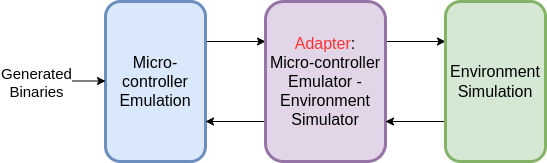
\includegraphics[width=14cm]{General concept.png}
    \label{fig: General concept}
\end{figure}
%---

In this undergraduate conclusion project, those three main problems will be approached. To do that, it will be used tools established in the industry with the goal to implement the micro-controller emulation and the environment simulation and design. Besides that, there is not any available tool capable of doing the interconnection between those features. 

% ----------------------------------------------------------
% MICROCONTROLLER
% ----------------------------------------------------------
\chapter{Micro-controller Emulation}

Embedded devices are projected with the main objective to execute specifics functions or to attend to a particular application, having, by definition, data processing capability. In that way, micro-controllers are widely used to achieve this goal. However, it is important to have clear understanding about they concept and functioning, due to the complexity and diversity of those chips.

\section{What is a Micro-controller}

As a whole, a micro-controller is a programmable embedded electronic device that integrates a processor, memory, and peripherals into a single integrated circuit. These devices have specific architectures depending on the manufacturer and feature a range of peripherals that perform specific functions.

Micro-controllers typically have 8, 16, or 32-bit architectures. Each architecture organizes information in memory differently, thereby altering, for example, the storage capacity of each address among many other things.

The peripherals of the micro-controller are responsible for communication between the micro-controller and the external world. They play a crucial role in receiving sensor information, managing communication interfaces, and sending signals, among other applications that result in actions in the external world.

Initially, the peripherals receive and send a series of electrical signals, which originate from various sensors and actuators, for example, that access internal circuits within the micro-controller, which in turn, modify the micro-controller's memory. Thus, when the micro-controller reads the information in memory, it realizes that the value has changed there and, if necessary, changes its output behavior.

In general, the peripherals receive and send a series of electrical signals from sensors and actuators, for example. These signals access internal circuits of the micro-controller, which can modify the device's memory. Therefore, when the micro-controller reads information from memory, it detects that the values have been modified and can change its output behavior accordingly.

%---
\begin{figure}[h]
\centering
    \caption{Micro-controller basic structure}
    \centering % para centralizarmos a figura
    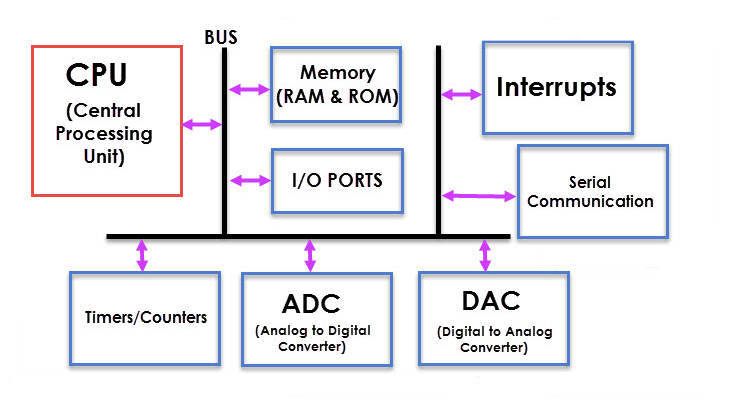
\includegraphics[width=14cm]{microcontroller_structure.png}
    \par
    Fonte: ElectronicsHub \cite{eletronic_hub_23}
    \label{fig: Micro-controller basic structure}
\end{figure}
%---


In the context of simulation, it is essential to replicate these external world functionalities, which are the responsibilities of the peripherals. Due to the specific way each peripheral accesses reserved positions in the micro-controller's memory and organizes information, it is important to explain in greater detail how this process is carried out for the peripherals that are the focus of emulation in this project.


\section{Memory and Peripherals of a micro-controller}
\subsection{General Purpose Input/Output (GPIO)}
The GPIOs (General Purpose Input/Output) are fundamental peripherals in micro-controllers, responsible for handling information in a binary form, represented as 0 or 1. In the context of micro-controllers, it is necessary to specify which PORT (port) and which PIN (pin) will be used to configure a particular GPIO. This appropriate selection allows for the allocation of the necessary pin within the circuit in which the micro-controller is integrated.

GPIOs function as MMOI (Memory Mapped Input/Output), meaning they map a specific memory location to store the information related to the PORT and PIN. Essentially, each port corresponds to a specific memory address, while each pin is a mask that indicates the memory position where the information is being stored.


%---
\begin{figure}[h]
\centering
    \caption{GPIO addresses from micro-controller STM32F103C8T6}
    \centering % para centralizarmos a figura
    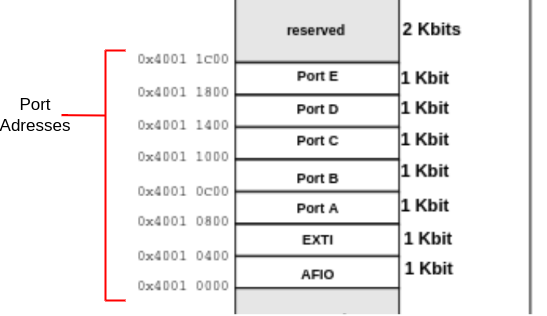
\includegraphics[width=14cm]{GPIO_addresses.png}
    \par
    Fonte: STM32F103C8T6 Datasheet \cite{STM32F103C8T6_Datasheet_23}
    \label{fig: GPIO addresses from micro-controller STM32F103C8T6}
\end{figure}
%---

Additionally, the configuration of the GPIO, such as determining whether it will be used as an input or output or for other functions, also influences the memory location that will be accessed to obtain the necessary information.


% \section{How to emulate a peripheral}


% ----------------------------------------------------------
% ENVIRONMENT
% ----------------------------------------------------------
\chapter{Environment Simulation}
\section{Modeling the environment}
The scope of modeling refers to how to simulation will look like. The two main objects that need to be modelled are: the room and the embedded system itself. To fulfill that objective, there are a variety of open-sources  software that provide modelling tools and are able to export the made objects to where the simulation will be run. 

\section{Running the environment}
The running environment integrates the modelled objects. It brings all the physical characteristics of both them and how they iterate with each other.In addition, the environment will be responsible to export and receive data to and from an external source.


% ----------------------------------------------------------
% INTEGRATION
% ----------------------------------------------------------
\chapter{Integration between the simulation and the emulation}
Nowadays there are many ways to make the interconnection and data exchange between between two different software.

For this project, it is necessary  a non-stop data exchange of both sides between the emulation and the simulation. To accomplish that, it is interesting to use used communication protocols that is shown as it follows:

\section{Protocol Buffers}
Protocol buffers \cite{google_protocol_buffers}, or protobufs, are mechanism developed by Google used to serialize different kind of data. Using a  language and platform neutral schema definition, protobufs are really useful to parse and serialize data between software that uses different types of languages and formats.

To define how the data will be structured, it is used the .proto files. These files needs to be compiled by the proto compiler to generate the source code structuring the data format in different types of languages. In that way, the same .proto file can used by different software.

%---
\begin{figure}[h]
\centering
    \caption{Protocol Buffer workflow}
    \centering % para centralizarmos a figura
    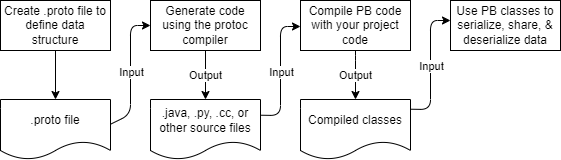
\includegraphics[width=14cm]{protobuf_workflow.png}
    \label{fig: protobuf_workflow}
\end{figure}
%---

Other important feature of this protocol is how their messages are compact. Using a compact binary format, it leads the application to less network load.

\section{Publishers and Subscribers}
This messaging pattern \cite{publisher_subscriber} is used to make the communication between different parts of a system or different software.

This pattern is based on what is called "topic", what is basically a channel that has two possible actions: to publish and to subscribe.

%---
\begin{figure}[h]
\centering
    \caption{Publisher-Subscriber Pattern}
    \centering % para centralizarmos a figura
    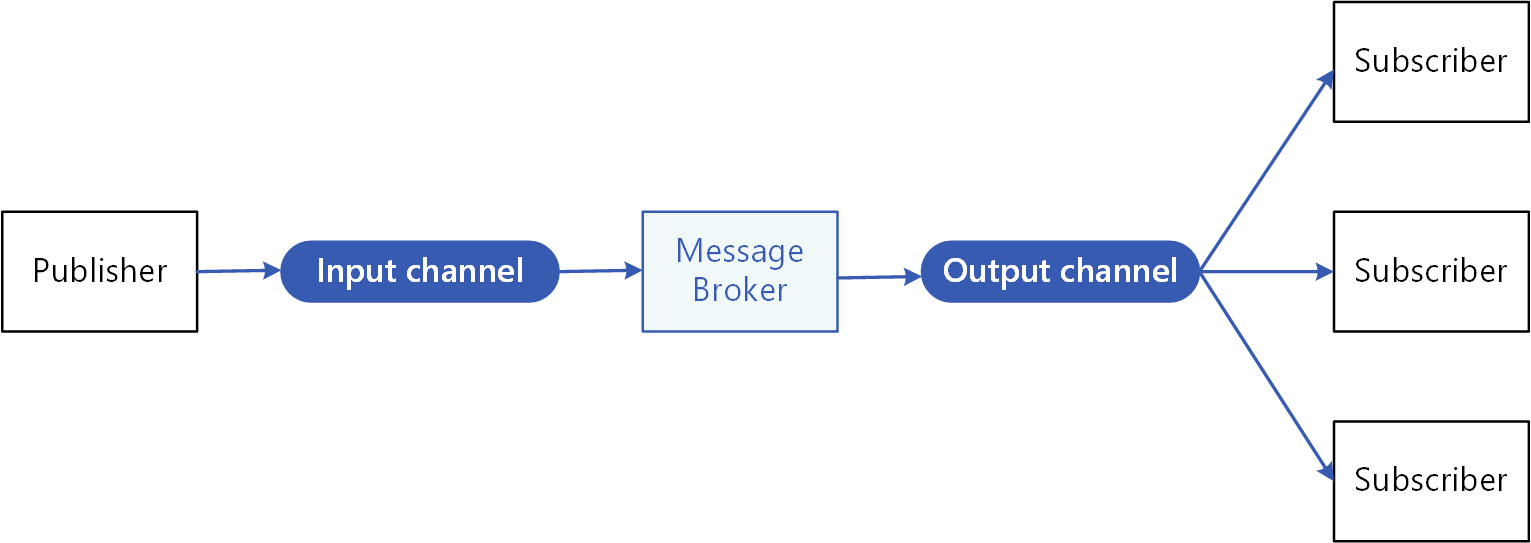
\includegraphics[width=14cm]{publish-subscribe.png}
    \label{fig: publisher subscriber pattern}
\end{figure}
%---

Publish, is to send a message to a topic. In other words, is to make that message visible to who has reading access to that topic, so it gives the topic data to be exchanged.

In the other hand, subscribe is to "listen" what is been published in a topic. As soon as the topic is published, the part which has subscribed to this topic receives a callback noticing the message's arrival and gets the data.

% ----------------------------------------------------------
% KVN AND EMULATION
% ----------------------------------------------------------
\chapter{KVN and Emulation}


\end{document}